\subsection{}

Remember ceteris paribus
\begin{definition}
    \emph{Law of Supply}, as the price of something goes up, your willingness to produce it goes up.
\end{definition}
\begin{definition}
    \emph{Quantity Supplied}
    \begin{itemize}
        \item The amount of a product that firms \emph{desire} to sell in some time period is called the \emph{quantity supplied}
        of that product.
        \item Quantity supplied is the amount that firms are willing to offer for sale and not necessarily the \emph{quantity actually sold}.
        \item Quantity supplied is a flow as opposed to a stock. 
    \end{itemize}
\end{definition}
\begin{definition}
    \emph{Supply Schedule} is a a table with prices and quantities (subscript s). Your willingness to produce
    a product should not go down as the price goes up. The quantity supplied depends on the price.
\end{definition}
\begin{definition}
    \emph{Supply Curve} is a graphical representation of the supply schedule. Price is on the y-axis and quantity on the x-axis.
    It is an upward sloping curve, it does not need to be linear. The supply curve is for the entire market for the product. 
    There exists a price where the quantity supplied is 0 (reservation price).
\end{definition}
\begin{definition}
    A \emph{shift} in supply is when other factors besides price change.\\
    A \emph{change in supply} is a change in quantity supplied at every price - a shift of the entire curve.\\
    A \emph{change in quantity supplied} refers to a movement from one point on a supply curve to another point - a
    movement along the supply curve.
\end{definition}
\begin{example}
    If price of inputs (resources) are increased, the supply curve shifts left.
\end{example}
\begin{figure}[h!]
    \centering
    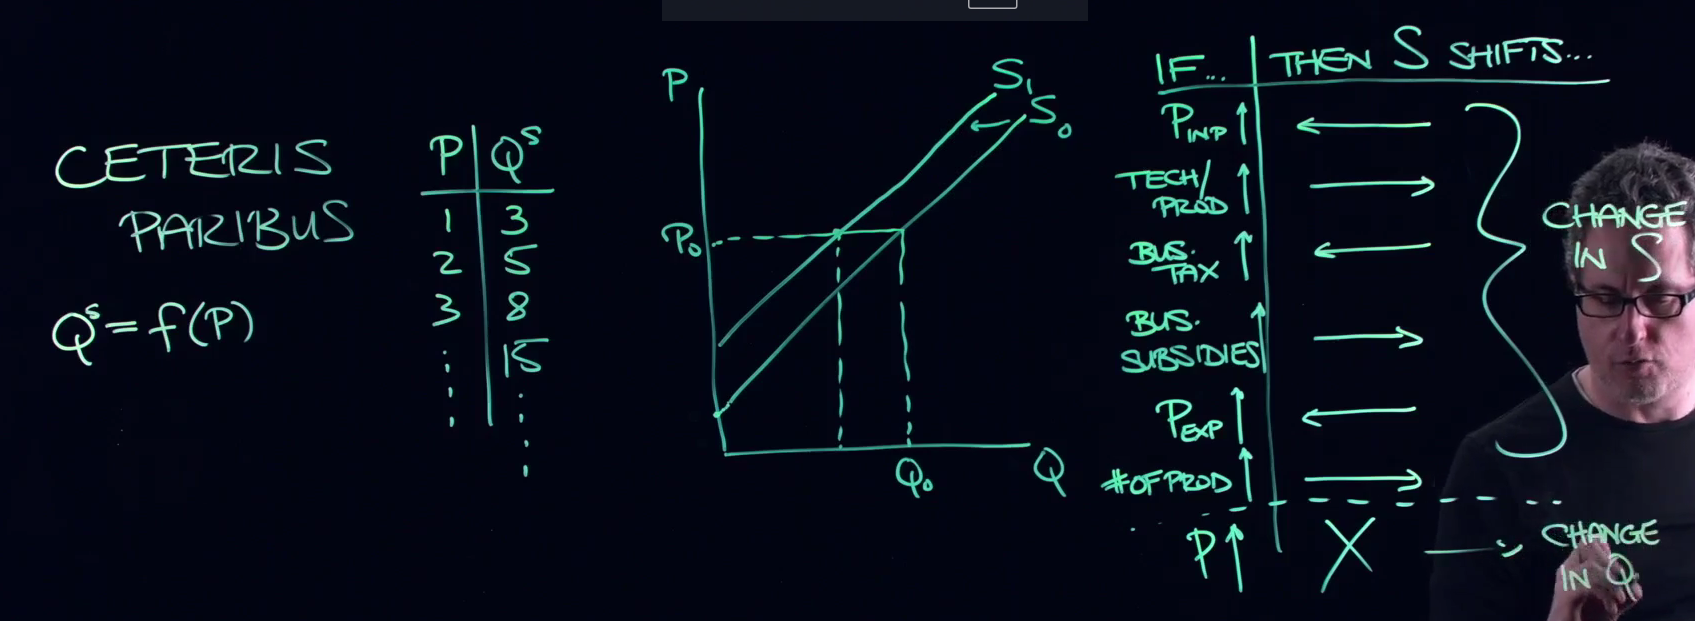
\includegraphics[width=\textwidth, height=\textheight, keepaspectratio]{Chapter3/Supply.png}
    \caption{Supply Information}
\end{figure}